\documentclass[a4paper,12pt,oneside,pdflatex,italian,final,twocolumn]{article}

\usepackage[utf8]{inputenc}
\usepackage{parallel}
\usepackage{siunitx}
\usepackage{booktabs}
\usepackage{fancyhdr}
\usepackage{subcaption}
\usepackage{listings}
\usepackage{hyperref}
\usepackage{pdfpages}

\usepackage[export]{adjustbox}
\usepackage[margin=0.5in]{geometry}
\addtolength{\topmargin}{0in}

\usepackage{libertine}
\renewcommand*\familydefault{\sfdefault}
\usepackage[T1]{fontenc}

\urlstyle{sf}
\hypersetup{
	colorlinks=true, %set true if you want colored links
	linktoc=all,     %set to all if you want both sections and subsections linked
	linkcolor=blue,  %choose some color if you want links to stand out
	urlcolor=blue,   %url color
}

\title{Cough Capture Manual}
\author{Achmadi ST MT}
\date{April 2023}

\begin{document}
	\pagestyle{fancy}

	\lhead{VibrasticLab}
	\chead{\today}
	\rhead{Specification Document v1.0}

	\onecolumn

	\begin{figure}

	\end{figure}\begin{minipage}{0.47\textwidth}
		\centering

	\end{minipage}
	\hfill
	\begin{minipage}{0.47\textwidth}
		\raggedleft
		\Huge \textbf{Cough Capture Manual}
	\end{minipage}

	\section{Requirements}

	\begin{itemize}
		\item Cough Capture Prototype Unit.

		\item Working Data Server.

		\item Working Wireless Local Area Network (WLAN).

		\item Laptop/Computer to access into Data server.
	\end{itemize}

	\raggedright
	\section{Cough Capture Unit}

	\centering
	\begin{figure}[!ht]
		\centering
		\includegraphics[width=\textwidth,]{images/proto_part.png}
		\caption{Prototype Unit}
	\end{figure}

	\raggedright
	Here general function of each part:

	\begin{itemize}
		\item \textbf{Power Source:} Powering the unit. Please use provided power adaptor unit.

		\item \textbf{Microphone Module:} For Audio Input. Please do not touch the microphone.

		\item \textbf{Button Trigger:} Tigger to Start Recording Session that last approximately 3 seconds.

		\item \textbf{Information Status:} Display Information Status:

		\begin{itemize}
			\item \textbf{Recording:} Show Recording Session. Either \textbf{Inactive} or \textbf{Active}.

			\item \textbf{Send Wav:} Show Data Sending to Server status. Either \textbf{Inactive} or \textbf{Active}.

			\item \textbf{Server:} Show Configured Server address. Please make sure the actual server already functional.

			\item \textbf{Edge-IP:} Show unit IP on configured WLAN. You can SSH access to unit using this IP with username \textbf{alarm} and no password.
		\end{itemize}

		\item \textbf{Audio Buffer Graph:} Show Audio Buffer for each 100 milliseconds. The axis are PCM amplitude and time in 100 ms span.
	\end{itemize}

	\raggedright
	\section{Server Data Access}

	In local area network, access the browser to address \url{http://10.124.3.221/signin}

	\centering
	\begin{figure}[!ht]
		\centering
		\includegraphics[width=\textwidth,]{images/web_signin.png}
		\caption{Data Server Login}
	\end{figure}
	\raggedright

	\textbf{NOTE:} If the Web doesnt loaded, possible problem:

	\begin{itemize}
		\item The Server Computer crash since it also used for Tensorflow processes in another projects

		\item The Server docker process still not started
	\end{itemize}

	Please contact the administrator if this does happen. Next, login using credential:

	\begin{itemize}
		\item \textbf{username:} admin@admin.com
		\item \textbf{password:} vibrastice101
	\end{itemize}

	\newpage
	\centering
	\begin{figure}[!ht]
		\centering
		\includegraphics[width=\textwidth,]{images/web_home.png}
		\caption{Data Server Home}
	\end{figure}
	\raggedright

	Next, Go to \textbf{Data Batuk Naracoba} from Side Tab:

	\centering
	\begin{figure}[!ht]
		\centering
		\includegraphics[width=\textwidth,]{images/web_datanarcob.png}
		\caption{Data Server Home}
	\end{figure}
	\raggedright

	Additional command button each data entry:

	\begin{itemize}
		\item \textbf{Cek Suara Batuk:} Check the Audio and Spectrogram of recorded

		\item \textbf{Edit Data:} To modify patient data such as names, genders, or ages.
	\end{itemize}

	\newpage
	\raggedright
	\section{Data Capture Procedure}

	Here step to capture the data:
	\begin{enumerate}
		\item Make sure the requirement in previous list already sufficient.

		\item Press and Release the \textbf{Trigger Button} on unit (Dont hold the Button).
		The \textbf{Recording} status become \textbf{Active}.

		\item For 3s, the unit will capture any audio, including cough audio.

		\item After recording over (Inactive status), the unit will try to send data to server.
		The \textbf{Send Wav} status become \textbf{Active}.

		\item If succeceded and all status become Inactive, refresh the browser to check new data entry.

		\item Edit the entry according the patient data by press \textbf{Edit Data}.
	\end{enumerate}

	\raggedright
	\section{Troubleshoot}

	If any problem, consult the project repository:

	\begin{itemize}
		\item Prototype Unit: \url{https://github.com/VibrasticLab/ehealth-iot/}

		\item Web Server: \url{https://github.com/VibrasticLab/ehealth-web/}
	\end{itemize}

	Or contact:

	\begin{itemize}
		\item Project Coordinator: \textbf{Roudhatul J.R, ST, MT} (+62-878-4480-0816)

		\item Project Staff: \textbf{M. Ammar A, ST} (+62-823-3028-0675)

		\item Server Maintainer: \textbf{A. Dwi P, ST} (62+857-0896-7654)
	\end{itemize}

\end{document}